\chapter{TiWM paradigm explored with MEG data}

 % Setup
 % - renvoyer au document de l'ensemble des choses que j'auraient aimés savoir dés le début

 % Deux études : 
 % - Welcome study
 % - Localizer ?
 % - Sample


 [résumer la situation et dire ce qu'il se passe dans ce chapitre. Raconter une histoire.]


Our exploration of the MEG data for the paradigm follows the classical steps of a MEG study:

\begin{itemize}
    \item Pre-Processing of the data. Our study started with the verification and cleaning of the data.
    \item Analysis in the sensor space. In this step we visualized the Evoked response of the different conditions. In order to find out when and how often the information is stored at the time of retrieval, we implemented a new procedure, based on Common Spatial Patterns (CSP). After determining the most salient time and frequency, we check the statistical significance of the response using cluster permutation tests.
          % \item [report visualization. CSP to see the patterns and see the frequencies and moments. Why at the beginning not at the end. We should have separated between the different length of sequence ??? Visualization of filters and paterns. Difficulties with the patterns. Should have taken just the first pattern].
    \item Source analysis. After having determined the frequency and the moment of maximum activation of the Working memory, we visualize the 3D response.
\end{itemize}


The \href{https://github.com/mne-tools/mne-bids-pipeline}{MNE-BIDS-Pipeline} is still in development. As I wanted to use it for the time in working memory paradigm, I had to help implement the missing features I needed. The list of features to which I contributed is presented in the table \ref{Tab:PR}.
% Ce chapitre détaille les modification liées à un probleme de recherche, 

\begin{table}[ht]
    \centering
    \begin{tabular}{@{}| p{3cm}|p{9cm}| @{}}
        \hline
        Type             & Title                                                                                                                                                                                                                                                                       \\
        \hline
        New feature      & Add possibility to exclude runs from the analysis via the new exclude run setting.                                                                                                                                                                                          \\
        Code health      & Files docstrings in the preprocessing steps were updated.                                                                                                                                                                                                                   \\
        Behavior changes & Warn if using ICA and no EOG- or ECG-related ICs were detected.                                                                                                                                                                                                             \\
        New feature      & Added the possibility to have different runs for different subjects.                                                                                                                                                                                                        \\
        Behavior changes & Check that the baseline interval falls into the epoch interval.                                                                                                                                                                                                             \\
        Behavior changes & ica\_reject now also applies to ECG and EOG epochs.                                                                                                                                                                                                                         \\
        Bug fix          & The sanity check comparing the rank of the experimental data and the rank of the empty-room after Maxwell-filtering did not use the maxfiltered data.                                                                                                                       \\
        Bug fix          & epochs\_tmin and epochs\_tmax were named incorrectly in some test config files.                                                                                                                                                                                             \\
        Bug fix          & We now reject bad epochs by using ica\_reject before producing the "overlay" plots that show the evoked data before and after ICA cleaning in the `proc-ica\_report`.                                                                                                       \\
        New feature      & It is now possible to analyze the contrast using the Common Spatial Patterns in the time-frequency domain using the new script: 03b-time\_frequency\_csp.py. We also test the significance of the contrast between the two conditions using cluster permutation statistics. \\
        \hline
    \end{tabular}

    \caption[Summary of my contributions to the MNE-BIDS-Pipeline.]%
    {Summary of my contributions to the MNE-BIDS-Pipeline on \href{https://raw.githubusercontent.com/mne-tools/mne-bids-pipeline/main/docs/source/changes.md}{GitHub}.}
    \label{Tab:PR}
\end{table}

\section{Preprocessing}

Before this internship, I had already worked on EEG data for the "Dream, sleep apnea" challenge or for the Kaggle "Inria - BCI Challenge". But on these two occasions, the data I had manipulated had already been cleaned by the competition organizers. This internship allowed me to realize the complexity of preprocessing data in brain imaging.

\subsection{presentations of the different stages}

The different phases of the data preprocessing are as follows:

[duplicates]

\begin{itemize}
    \item Finding bad channels: some channels of MEG recordings may be noisy or flat. They need to be identified and marked as bad so they are not taking into account during the analysis;
    \item Applying Maxwell filter : help to remove part of the sensors noise;
    \item Frequency filter: to remove non desired frequency bands;
    \item Creating epochs: epochs are data structures to represent equal-duration chuncks of MEG signals. When the recording session includes stimuli, epochs are often defined from 0.2 seconds before the stimulus to 0.5 seconds after. Otherwise, like in rest session, epochs are fixed and overlapping frames of the MEG signal.
    \item Computing evoked data: they are created by averaging MEG signal over several epochs. It is useful to study stimulus-evoked brain activity.
\end{itemize}


The figure \ref{cheat_sheet} summarizes the preprocessing step in the pipeline. At the beginning of my internship, I created this table in order to familiarize myself with the different scripts of the pipeline. Then, I added the main problems that occur in practice associated with each step as well as the main ideas of sanity checks to be performed after the execution of the pipeline.

\begin{figure}[ht]
    \centering
    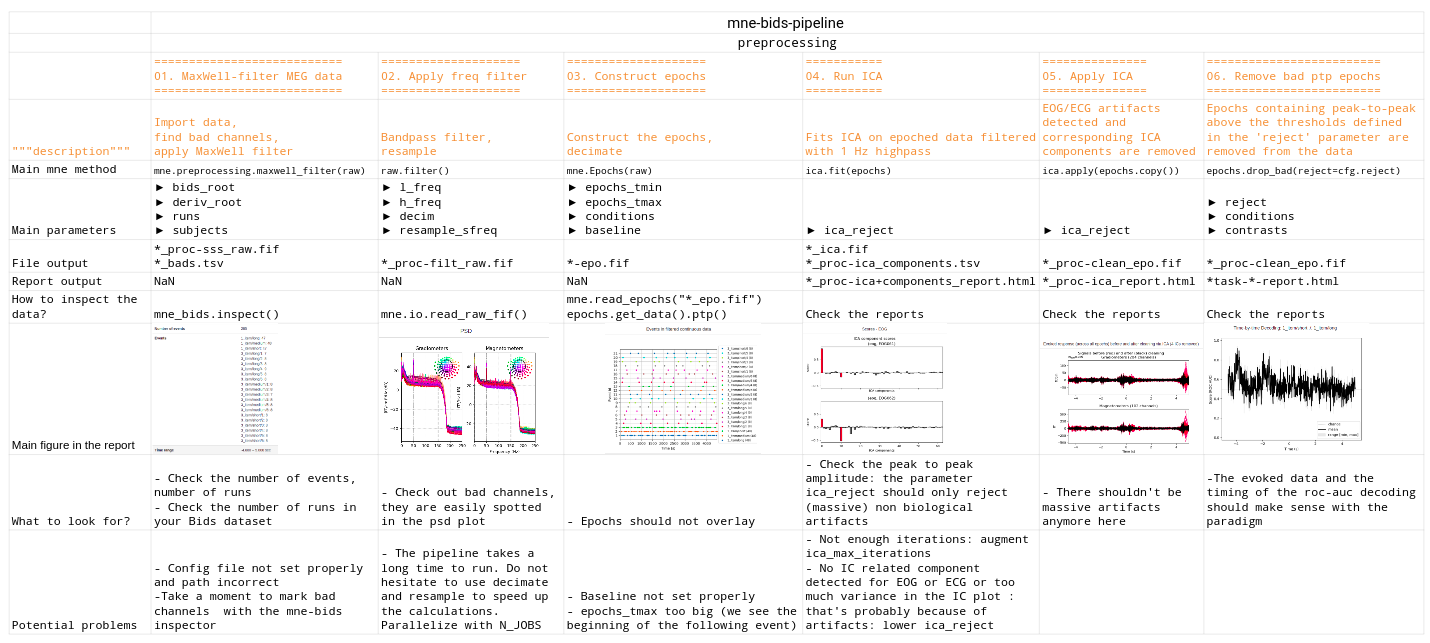
\includegraphics[width=15cm]{images_report/preprocessing/cheatsheet preprocessing.png}
    \caption[Summary of the preprocessing of the pipeline.]%
    {Summary of the preprocessing of the pipeline.}
    \label{cheat_sheet}
\end{figure}


% \subsection{Bids Pipeline}
% - Premiereres PR necessité pourquoi ?
% premiere contri open source
% avec une utilité

% Lors de l'étape du preprocessing au début de mon stage, il a fallut que je me familiarise avec la librairie mne-bids-pipeline et tous ses différents script, et également afin de me familieariser avec le developpement open-source ainsi que les exigences qui en découlent.

% Mes premieeres contributions consistere donc à rajouter des sanity check dans la pipeline, actualiser les docstring et les en tetes de codes, travailler sur l'hormonie du code en harminisant les noms des variables entre les différents scripts.

\subsection{Preprocessing of artifacts}
\label{preprocessing_of_artifacts}


\begin{figure}[ht]
    \centering
    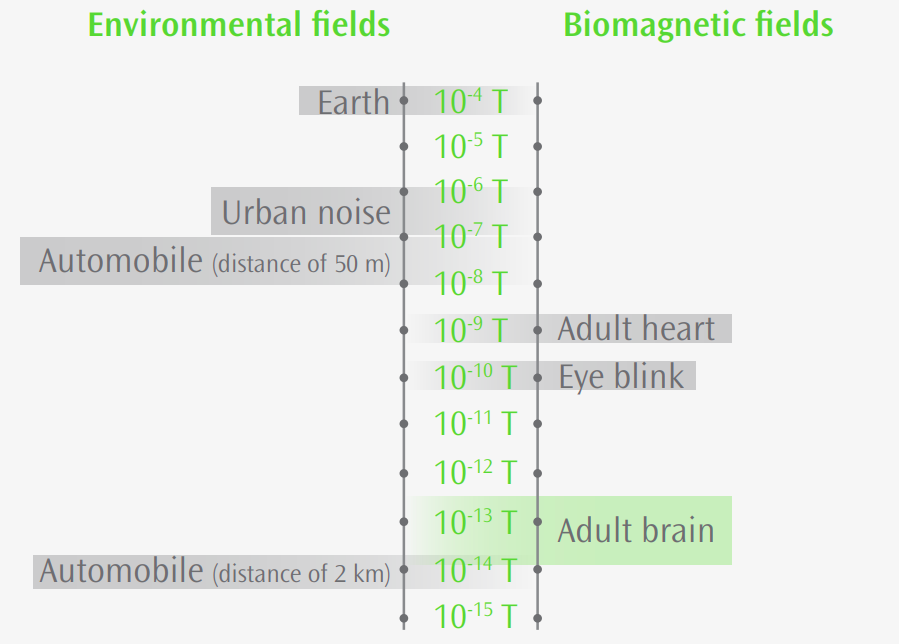
\includegraphics[width=7cm]{images_report/sensor/noise_order_of_magnitude.png}
    \caption[Scale of magnitude of different magnetic fields]%
    {Scale of magnitude of different magnetic fields}
    \label{noise_order_of_magnitude}
\end{figure}


An important point is the order in which the data is rejected. Indeed, a major difficulty with raw data coming from cortical signals is the fact that these signals are extremely small. Although the data is recorded in a shielded chamber, the slightest noise can totally overwhelm the signal. Figure \ref{noise_order_of_magnitude} shows the scale of orders of magnitude, which makes it clear that the external noise is of an order of magnitude immeasurably larger than the neurological signals of interest.

Even after removing all the noise from the external environment, some of the so-called biological artifacts, such as heartbeats and blinks, must be removed by either discarding the contaminated time interval or separating the sources by using independent component analysis (ICA), which separates the heartbeat and blink sources from the rest of the signal.

The figure \ref{rejection_pipeline} allows to visualize the pipeline rejection of the mne-bids-pipeline.

\begin{figure}[ht]
    \centering
    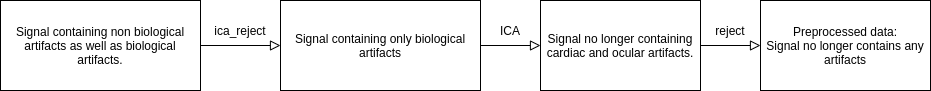
\includegraphics[width=15cm]{images_report/preprocessing/rejection_pipeline.png}
    \caption[Simplification of the BIDS-Pipeline rejection process.]%
    {Simplification of the BIDS-Pipeline rejection process.}
    \label{rejection_pipeline}
\end{figure}

Here are the details of the procedure:
\begin{itemize}
    \item At the beginning the signal contains both biological artifacts (eye blink, heartbeat), and non biological artifacts. The latter are of an order of magnitude larger than the biological artifacts.
    \item We can start by filtering the different epochs using rejecting the epochs whose peak-to-peak amplitude exceeds the amplitude specified by the "ica\_reject" parameter. This parameter allows to filter signals that are 50 times larger than the nominal amplitude and therefore allows to make a first screening.
    \item The resulting signal does not contain any more redhibitory non-biological artifact, which allows to improve the convergence of the ICA, allowing to separate the sources for the ocular and cardiac artifacts.
    \item The ICA source separation does not work perfectly, so an additional step is required to reject the last artifacts using the "reject" parameter, which allows to filter the signals with a peak-to-peak amplitude 10 times higher than the nominal amplitude. The result is the preprocessed signal.
\end{itemize}

Even if the global pipeline rejection method was already established before my arrival, the experimental data revealed problems in the order of the filtering operations, and we thus improved a lot the automatic data preprocessing especially for difficult data that contains simulaneously biological and non-biological artifacts such as phase inversion fields. Figure \ref{fig:PR_ica} shows an example of ICA enhancement before and after our Pull request that changes the order of operations, in particular by filtering out non-biological signals before the ICA.


\begin{figure}
    \centering
    \begin{subfigure}{.5\textwidth}
        \centering
        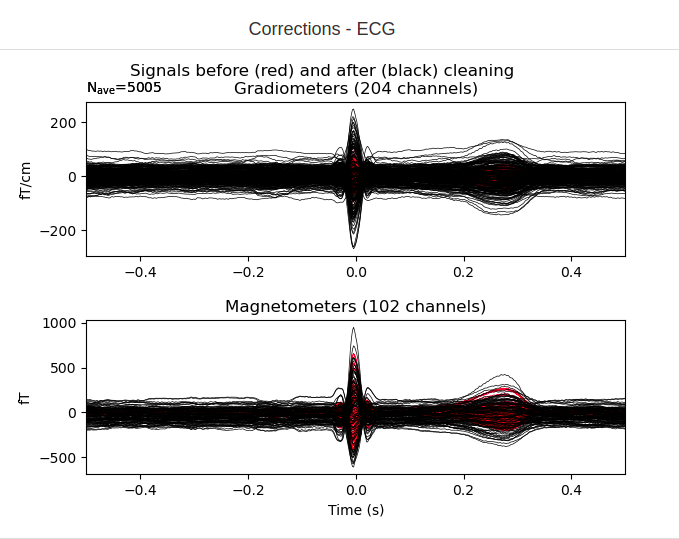
\includegraphics[width=1.\linewidth]{images_report/preprocessing/ica/ECG_ICA_before_PR.png}
        \caption{ICA correction before amelioration}
        \label{fig:before_ica_PR}
    \end{subfigure}%
    \begin{subfigure}{.5\textwidth}
        \centering
        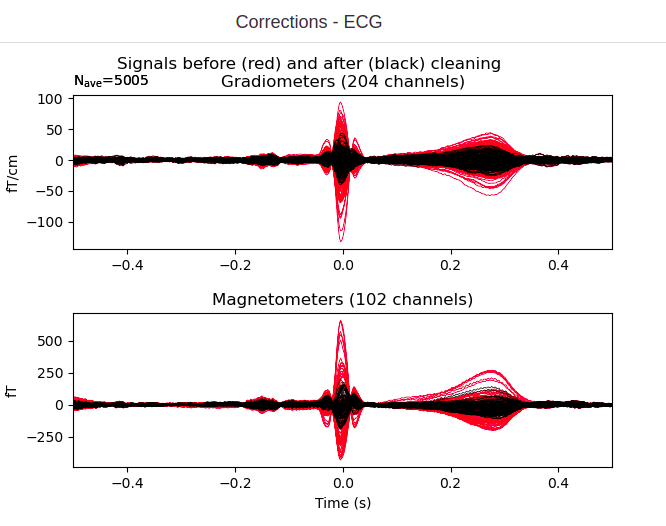
\includegraphics[width=1.\linewidth]{images_report/preprocessing/ica/ECG_ICA_after_PR.png}
        \caption{ICA correction after amelioration}
        \label{fig:after_ica_PR}
    \end{subfigure}
    \caption{We can see that after amelioration, we no longer obtain a discontinuity, and the ICA is capable of reducing almsot by 4 the peak to peak amplitude of the ECG artifact.}
    \label{fig:PR_ica}
\end{figure}



[put an example of a heart or EOG ? Example of preprocessing reports.].

\section{Analysis in Sensor Space}

\subsection{Insufficiency of the pipeline to analyze in a relevant way the MEG}

\begin{figure}[htb]
    \centering % <-- added
    \begin{subfigure}{0.25\textwidth}
        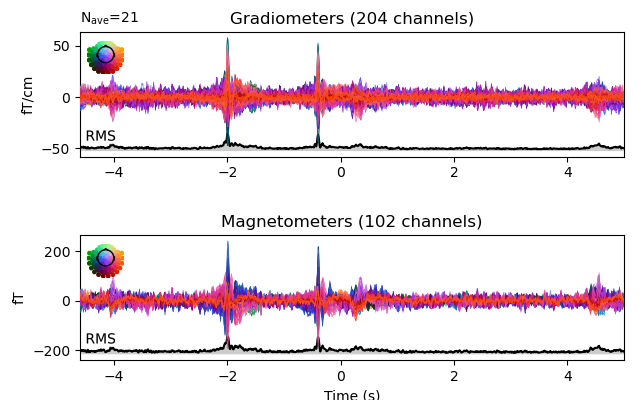
\includegraphics[width=\linewidth]{images_report/sensor/evoked/1_item_short.png}
        \caption{1\_item\_short}
        \label{fig:1_item_short}
    \end{subfigure}\hfil % <-- added
    \begin{subfigure}{0.25\textwidth}
        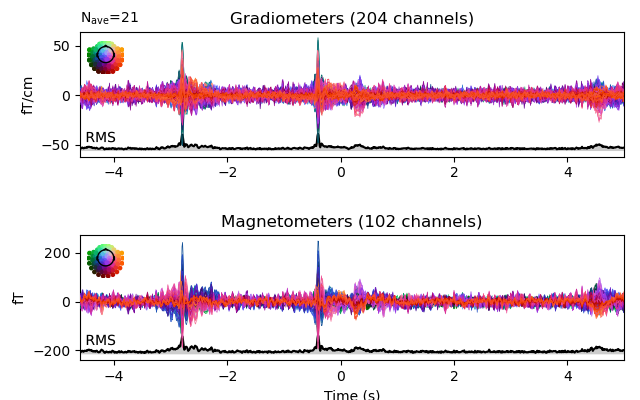
\includegraphics[width=\linewidth]{images_report/sensor/evoked/1_item_medium.png}
        \caption{1\_item\_medium}
        \label{fig:1_item_medium}
    \end{subfigure}\hfil % <-- added
    \begin{subfigure}{0.25\textwidth}
        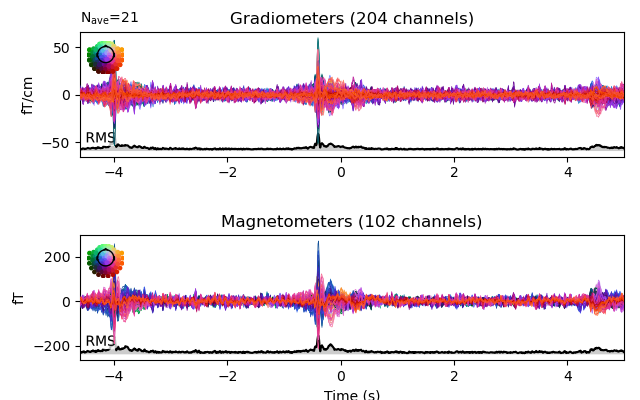
\includegraphics[width=\linewidth]{images_report/sensor/evoked/1_item_long.png}
        \caption{1\_item\_long}
        \label{fig:1_item_long}
    \end{subfigure}

    \medskip
    \begin{subfigure}{0.25\textwidth}
        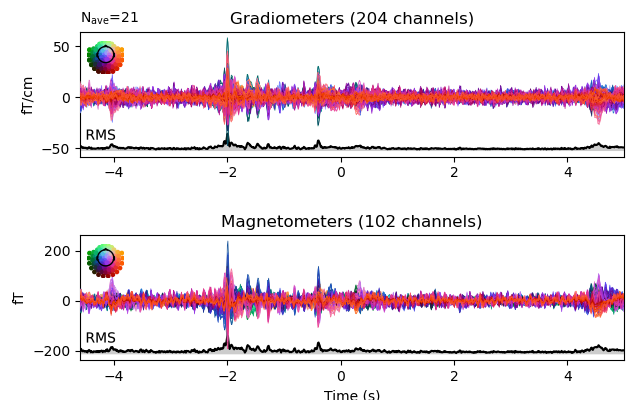
\includegraphics[width=\linewidth]{images_report/sensor/evoked/3_item_short.png}
        \caption{3\_item\_short}
        \label{fig:3_item_short}
    \end{subfigure}\hfil % <-- added
    \begin{subfigure}{0.25\textwidth}
        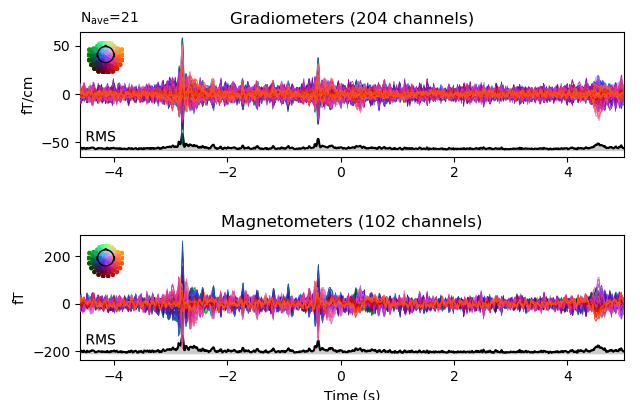
\includegraphics[width=\linewidth]{images_report/sensor/evoked/3_item_medium.png}
        \caption{3\_item\_medium}
        \label{fig:3_item_medium}
    \end{subfigure}\hfil % <-- added
    \begin{subfigure}{0.25\textwidth}
        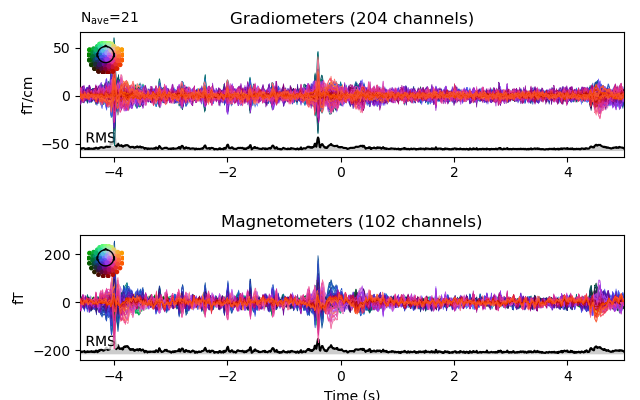
\includegraphics[width=\linewidth]{images_report/sensor/evoked/3_item_long.png}
        \caption{3\_item\_long}
        \label{fig:3_item_long}
    \end{subfigure}
    \caption[Evoked data for our 6 different items.]%
    {Evoked data for our 6 different items.}
    \label{fig:Evoked_data}
\end{figure}


\begin{figure}
    \centering
    \begin{subfigure}{.5\textwidth}
        \centering
        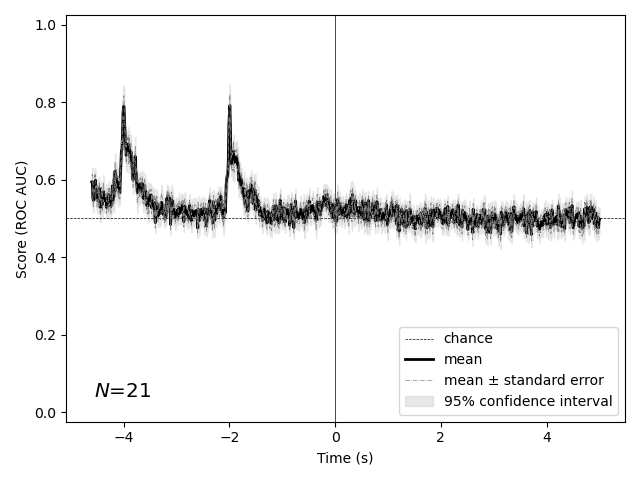
\includegraphics[width=1.\linewidth]{images_report/sensor/contrast/contrast_1_item_short_vs_1_item_long.png}
        \caption{Decoding between 1\_item\_short and 1\_item\_long.}
        \label{fig:decoding_1_item}
    \end{subfigure}%
    \begin{subfigure}{.5\textwidth}
        \centering
        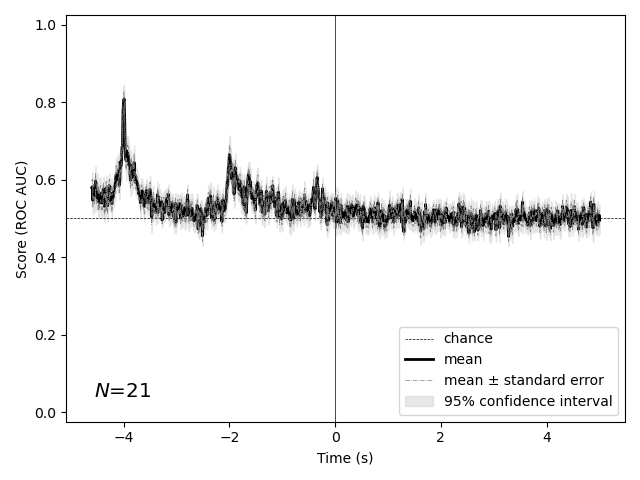
\includegraphics[width=1.\linewidth]{images_report/sensor/contrast/contrast_3_item_short_vs_3_item_long.png}
        \caption{Decoding between 3\_item\_short and 3\_item\_long.}
        \label{fig:decoding_3_item}
    \end{subfigure}
    \caption{Decoding ititialement dans la pipeline.}
    \label{fig:decoding_initial}
    % mettre seulement 1item vs 3 item ici
\end{figure}

\begin{figure}[ht]
    \centering
    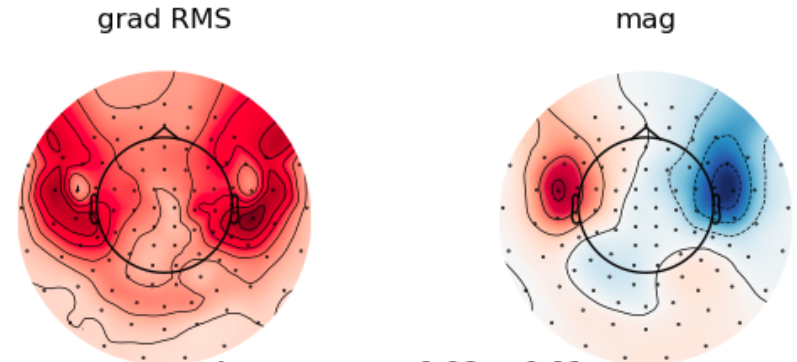
\includegraphics[width=9cm]{images_report/sensor/auditory_cortex.png}
    \caption[Topographic map of the first peak from 1\_item\_short.]%
    {Topographic map of the first peak from 1\_item\_short evoked data \ref{fig:1_item_short}. We can see that during these peaks which appear on the figures \ref{fig:Evoked_data}, it is above all the auditory cortex which is involved.}
    \label{auditory_cortex}
\end{figure}

At the beginning of my internship, the mne-bids-pipeline allowed us to quickly obtain figures such as \ref{fig:Evoked_data} and such as \ref{fig:decoding_initial}. These figures show that the preprocessing went well since the results are clean. But these two figures also present some limits in the framework of our paradigm.

- The figure \ref{fig:Evoked_data} presents the evoked data for each of our 6 different items. The three top figures are temporal sequences containing only one interval (1 item), while the three bottom figures contain sequences of 3 intervals (3 items). 
When there is only one item, we observe two very clear peaks before $t \leq 0$. These two peaks correspond to the pure tone which give the beginning and the end of the interval. After $t \geq 0$ begins the restitution phase, i.e. the phase during which the participant must recall the sequence in his head as precisely as possible. We see that during this restitution phase, the evoked data does not present any particular phenomenon, there is no peak to exploit. 

- In the same way for the figure \ref{fig:decoding_initial}, even if we can see that the decoder used in the pipeline manages to decode the signals before $t=0$ in a very satisfactory way, especially at the location of the auditory stimuli, the performance of the decoders is null during the restitution phase.

In this study, we are not interested in the auditory cortex, but in the working memory. We must therefore concentrate not on the listening phase before $t \leq 0$, but rather on the restitution phase after $t \geq 0$. This means that the algorithms currently in place in the pipeline were not sufficient at the beginning of my internship, and that we must find an adequate method to study the working memory.

\subsection{Strategy: analysing the contrast in time-frequency space}

Classically the sensor space is decomposed in the following steps:
\begin{itemize}
    \item creation of the evoked data sets are created by averaging different conditions.
    \item Using a sliding estimator with a logistic regression model for every time point.
    \item Time frequency decomposition: the epoched data is transformed to time-frequency domain.
    \item Computation of the group average results.
\end{itemize}

This order of operations is fine for most studies. But in the case of our study it is crucial to obtain results in the time-frequency space. We therefore need to combine the features of the "sliding estimator" script to study a contrast between two conditions and the "time frequency decomposition" script to study the signal in time and frequency space. It is to fill this gap that I implemented a new script in the pipeline allowing to visualize which are the time-frequency bin which present in the most salient way the working memory by studying the contrast between the sequences of an item and the sequences of 3 items. 

Indeed, 3\_items load the working memory much more than a single item. The reason for contrasting 3\_items with 1\_item and not 3\_item with 0\_item (rest) is that the contrast should not be based on a difference in the nature of the tasks, but rather a difference in load.

My \href{https://github.com/mne-tools/mne-bids-pipeline/pull/414}{pull request} adds a new script to the pipeline, designed to analyze in the time-frequency domain a contrast between two conditions. There are two main steps in this script:
\begin{enumerate}
    \item Decoding: for each time-frequency bin: For each time-frequency bin, we use a csp classifier in order to distinguish between the two conditions. We compute the roc-auc score for each time-frequency bin.
    \item Permutation statistics at the group level: We try to answer the following question: is the difference between the two conditions statistically significant? We use the classic permutations cluster tests on the time-frequency roc-auc map.
\end{enumerate}

\subsection{Decoding with Common Spatial Patterns (CSP)}

The time-frequency decomposition is estimated by iterating over raw data that has been band-passed at different frequencies. This is used to compute a
covariance matrix over each epoch or a rolling time-window and extract the CSP
filtered signals. A linear discriminant classifier is then applied to these
signals.

CSP is a technique to analyze multichannel data based on recordings from two classes qui a été introduite dans le contexte des EEG par \cite{koles1990spatial}.

\subsubsection{Intuitive explanation}

% Why CSP better than ...

I took the figure from \cite{blankertz2007optimizing} which also contains a conprehensive tutorial on CSP.

\begin{figure}
    \centering
    \begin{subfigure}{.5\textwidth}
        \centering
        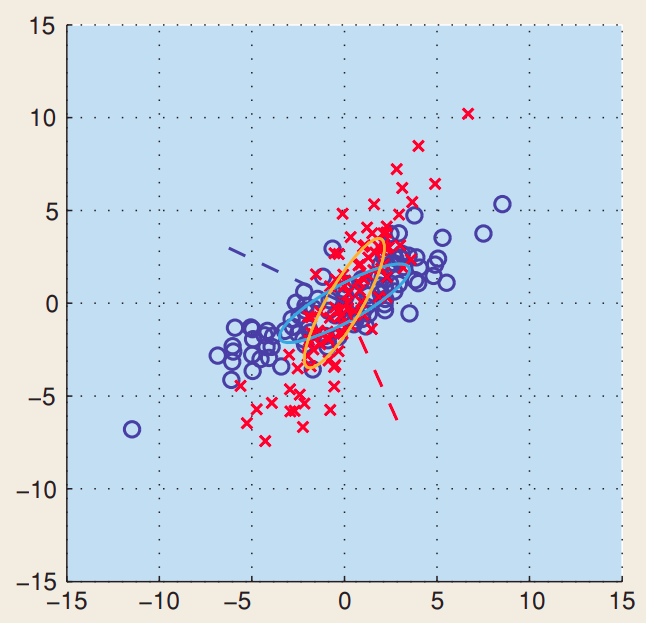
\includegraphics[width=1.\linewidth]{images_report/sensor/before_csp_filtering.png}
        \caption{Before CSP filtering}
        \label{fig:before_csp}
    \end{subfigure}%
    \begin{subfigure}{.5\textwidth}
        \centering
        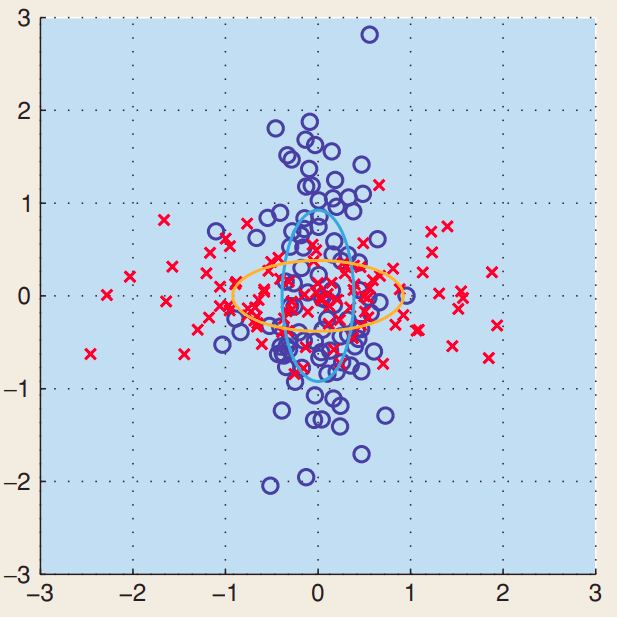
\includegraphics[width=1.\linewidth]{images_report/sensor/after_csp_filtering.png}
        \caption{After CSP filtering}
        \label{fig:after_csp}
    \end{subfigure}
    \caption{Toy example showing the functioning of the CSP transformation.}
    \label{fig:csp_intuitive}
\end{figure}
[je peux faire un shema mieux]

If we have two Gaussian signals, both centered in zeros, but with different principal directions, we can try to transform the two scatterplots in such a way that the principal directions of the two scatterplots in the CSP space are orthogonal so as to maximize the ratio of the variances following the principal directions.

For example on the figure \ref{fig:csp_intuitive}, we start from two point clouds, red and blue, very correlated, which we transform into decoupled red' and blue' point clouds.

The main vector of the red' cloud is aligned on the absice axis, while the main vector of the blue' cloud is aligned on the ordinate axis.

By this process, we maximize the variance ratio along the abscissa axis between the red' and the blue' clouds.

In our usage, a point cloud corresponds to an event, and each color corresponds to a different condition. Here, we do not try to classify points individually as in machine learning, but we classify a whole point cloud. If we try to guess the color/condition of a point cloud, we just have to transform the point cloud with the same transformation as before (i.e. apply the unmixing matrix as we will see later), and take the projection on the x axis of the new point cloud. We can then calculate the variance along the x axis and then train a linear classifier to discriminate among the different variances. By combining the csp algorithm, and for example a logistic regression, we can classify between the two conditions.

\subsubsection{Technical Description}

The above explanation only explains intuitively the algorithm for the first component of the CSP. But it does not explain how to obtain the other orientations. An efficient formulation to obtain all components of the CSP while being computationally reasonable is to formalize the problem as a generalized eigenvector problem.
[mettre les deux autres formulations]

\paragraph{General Eigenvalue Problem Formulation}

Let $X \in \mathbb{R}^{C * T}$ be a matrix containing $C$ channels and $T$ time points. The data at a single time point is denoted by $x(t) \in  \mathbb{R}^{C}$. Common spatial pattern (CSP) finds a decomposition that projects the signal in the original sensor space to CSP space using the following transformation:

\begin{equation}
    x_{\text{CSP}}(t) = W^{T}x(t)
\end{equation}

where each column of $W \in \mathbb{R}^{C*C}$ is a spatial filter and each row of $x_{\text{CSP}}(t)$ is a CSP component. Let $\Sigma^{+} \in \mathbb{R}^{C * C}$ and $\Sigma^{-} \in \mathbb{R}^{C * C}$ be the respective covariance matrices of the two different conditions. CSP analysis is given by the simultaneous diagonalization of the two covariance matrices.


\begin{equation}
    W^{T} \Sigma^{+} W = \lambda^{+}
    \label{eq:lambda_plus}
\end{equation}
\begin{equation}
    W^{T} \Sigma^{-} W = \lambda^{-}
    \label{eq:lambda_minus}
\end{equation}

Where the two $\lambda$ are diagonal matrices whose entries are the eigenvalues of the following generalized eigenvalue problem in $(w, \lambda) \in (\mathbb{R}^{C}, \mathbb{R})$:

\begin{equation}
    \Sigma^{+} w = \lambda \Sigma^{-} w
    \label{eq:general_eigenvalue}
\end{equation}

Large entries in the diagonal matrix corresponds to a spatial filter which gives high variance in one class but low variance in the other. Thus, the filter facilitates discrimination between the two classes.

\paragraph{The unmixing matrix}

Une autre manière de lire les deux equations \ref{eq:lambda_plus} et \ref{eq:lambda_minus} est de se rappeller que $w^{T}\Sigma w$ calcule la variance de la covariance $\Sigma$ suivant la direction $w$. Ainsi, $W^{T} \Sigma^{+} W$ et $W^{T} \Sigma^{-} W$ ne font que calculer des matrices diagonales, dont les elements diagonaux sont les variances des covariances suivant les différentes colonnes de $W$, à savoir les variances suivant les difféntes filtres spatiaux.

En trouvant tous les $w$ qui satisfont l'équation \ref{eq:general_eigenvalue}, on construit ainsi la matrice $W$ aussi appellée \textit{unmixing matrix}.

Apres avoir trouvé tous les couples $(w_i, \lambda_i)$ qui satisfont l'équation aux valeurs propres généralisées \ref{eq:general_eigenvalue}, on peut ordonner les solutions par valeurs propres décroissantes. Le premier filtre correspond à la direction maximisant le rapport des variances entre les deux nuages de points. En effet, si l'on remplace dans l'équaqtion \ref{eq:lambda_plus}, \ref{eq:lambda_minus}, on obtient:

\begin{equation}
    w^{T}_{i} \Sigma^{+} w_{i} = \lambda^{+}_{i}
    \label{eq:lambda_plus_first_component}
\end{equation}
\begin{equation}
    w^{T}_{i} \Sigma^{-} w_{i} = \lambda^{-}_{i}
    \label{eq:lambda_minus_first_component}
\end{equation}

Et il suffit alors de remplacer dans \ref{eq:general_eigenvalue} puis de multiplier à gauche par $w^{T}$ pour obtenir

\begin{equation}
    \lambda_1 = \lambda^{+}_1 / \lambda^{-}_1
\end{equation}

% complement eventuel
% https://www.youtube.com/watch?v=S4znknOIcRk&t=332s
% https://www.youtube.com/watch?v=zsOULC16USU

\subsection{Significance of time-frequency bins with Permutation statistics}

We try to answer the following question: is the difference between
the two conditions statistically significant? We use the a permutations
cluster tests on the time-frequency roc-auc map in order to check the significance of the activation.

\subsubsection{Overview of the cluster permutation statistics method}

\begin{figure}[ht]
    \centering
    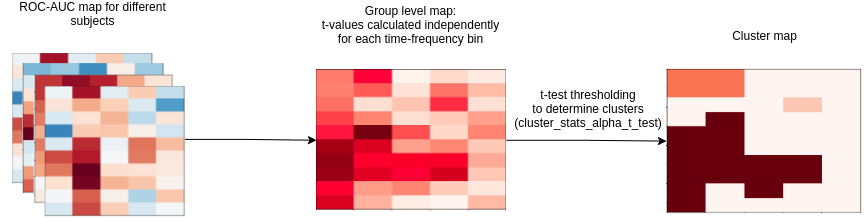
\includegraphics[width=15cm]{images_report/sensor/Permutation_statistics.png}
    \caption[Overview of the permutation statistics pipeline.]%
    {Overview of the permutation statistics pipeline.}
    \label{permutation_statistics_pipeline}
\end{figure}

La figure \ref{permutation_statistics_pipeline} donne un apercut de la pipeline de création des clusters.

On commence par rassembler toutes les time-frequency roc-auc map de tous les sujets. Pour chaque time-frequency bin, on calcule une t-value, de manière indépendante pour chaque bin (le détail des calculs se trouve en annexe). On obtient anisi la carte des t-values. Puis afin de trouver l'emplacement des clusters, il suffit d'utiliser un seiuil, par exemple correspodant à un niveau de chance de $0.05$ ou de $0.01$. Ce seil n'a pas une grande importance mathématique, mais en pratique, il permet de controler la taille des clusters. Une fois le seuil appliqué, on obtient potentiellement un ou des clusters. Afin de pouvoir attribuer une p-valeurs à chaque cluster, il faut alors utiliser le mécanismes des permutations.

Le mécanisme des permutation consiste à caluler une métrique sur nos cluster: qui peut être classiquement soit la taille du cluster, soit le maximum de t-vleur au sein du cluster, soit la somme des t-valeur au sein du cluster. Puis on compare cette métrique à la distribution de cette métrique simulée pour les permutation:
On inverse le signe de la différence pour chaque bin de chaque subject. On obtient la distribution de la metrique dans l'hypothese nulle ou The distribution of spatial cluster sizes is independent of the sign of the data.


\subsection{Implementation}



\subsection{Results}
- Discussion
- resultats significatifs alors que dans la tête


\subsection{Limites + Discu}

- Seuelemnt 2 classes

\section{Source Space Analysis}

- Generalités source space
Nouveau script: Contrast in source space
- Motivation : Insuffiscance de pipeline classique
- faire le Schéma
- Results:
- Interpretation sur Freeview
- Discussion
- Annexes : Subtilité :
Neuroscience : quest ce qui constitue du bruit ? Quel choix de la matrice de covariance
Subtilités mathématiques :  commutativité Log + moyenne
Limites:
